\documentclass[10pt,aspectratio=169]{beamer}

% All the boilerplate is in deslides.sty
\usepackage{deslides}

\author{Ji\v{r}\'i Lebl}

\institute[OSU]{%
Oklahoma State University%
%Departemento pri Matematiko de Oklahoma {\^S}tata Universitato%
}

\title{First order linear PDE\\(Notes on Diffy Qs, 1.9)}

\date{}

\begin{document}

\begin{frame}
\titlepage

%\bigskip

\begin{center}
The textbook: \url{https://www.jirka.org/diffyqs/}
\end{center}
\end{frame}

\begin{frame}
Consider the first order linear PDE problem
\begin{equation*}
a(x,t) \, u_x + b(x,t) \, u_t + c(x,t) \, u = g(x,t), \qquad u(x,0) = f(x) , \qquad -\infty < x < \infty,
\quad t > 0 ,
\end{equation*}
\pause
$u(x,t)$ is a function of $x$ and $t$.

\medskip
\pause

\emph{initial condition} $u(x,0) = f(x)$ is a function of $x$.

\medskip
\pause

We will describe the \emph{method of characteristics}:
find lines along which the equation is an ODE.

\end{frame}

\begin{frame}
\textbf{Example} (Transport equation)\textbf{:}
Consider
\quad $u_t + \alpha u_x = 0$, \quad $u(x,0) = f(x)$.

\medskip
\pause

We change to so-called \emph{characteristic coordinates} $(\xi,s)$.

\medskip
\pause

In this case:
\qquad $\xi = x - \alpha t$,  \quad $s = t$.

\medskip
\pause

Compute
\[
u_t = u_\xi \xi_t + u_s s_t \pause = - \alpha u_\xi + u_s ,
\qquad
\pause
u_x = u_\xi \xi_x + u_s s_x \pause = u_\xi .
\]
\pause
The equation becomes
\[
\underbrace{(- \alpha u_\xi + u_s)}_{u_t} + \alpha
\underbrace{(u_\xi)}_{u_x} = 0 ,
\pause
\qquad\text{or}\qquad
u_s = 0 .
\]
\pause
Treating $\xi$ as a parameter, we have an ODE
\quad $\dfrac{d u}{d s} = 0$.
\end{frame}

\begin{frame}
Solution is a function not depending on $s$:
\qquad 
$u = A(\xi) \pause = A(x - \alpha t)$

\medskip
\pause

Initial condition says:
\qquad
$f(x) = u(x,0) \pause = A(x - \alpha 0) \pause = A(x)$ \pause \wthus $A=f$.

\pause
\medskip

\thus \qquad
$u(x,t) = f(x-\alpha t)$.

\medskip
\pause

Curves given by
$\xi = \text{constant}$ are called the
\emph{characteristics}.

\medskip
\scalebox{0.9}{\subimport*{../figures}{char-curves.pdf_t}}
\end{frame}

\begin{frame}

In the $(x,t)$ coordinates, the characteristic curves satisfy 
$t = \frac{1}{\alpha} ( x- \xi)$, and are in fact lines.
The slope of characteristic lines is
$\frac{1}{\alpha}$, and for each different $\xi$, we get a different
characteristic line.

We see why $u_t + \alpha u_x = 0$ is called the
transport equation: Everything travels at some constant speed.
This behavior is called \emph{convection}.
An example application is material being moved by a river where the material
does not diffuse and is simply carried along.  In this setup, $x$ is 
the position along the river, $t$ is the time, and $u(x,t)$ the concentration the
material at position $x$ and time $t$.  See
{fopde:transportfig} for an example.

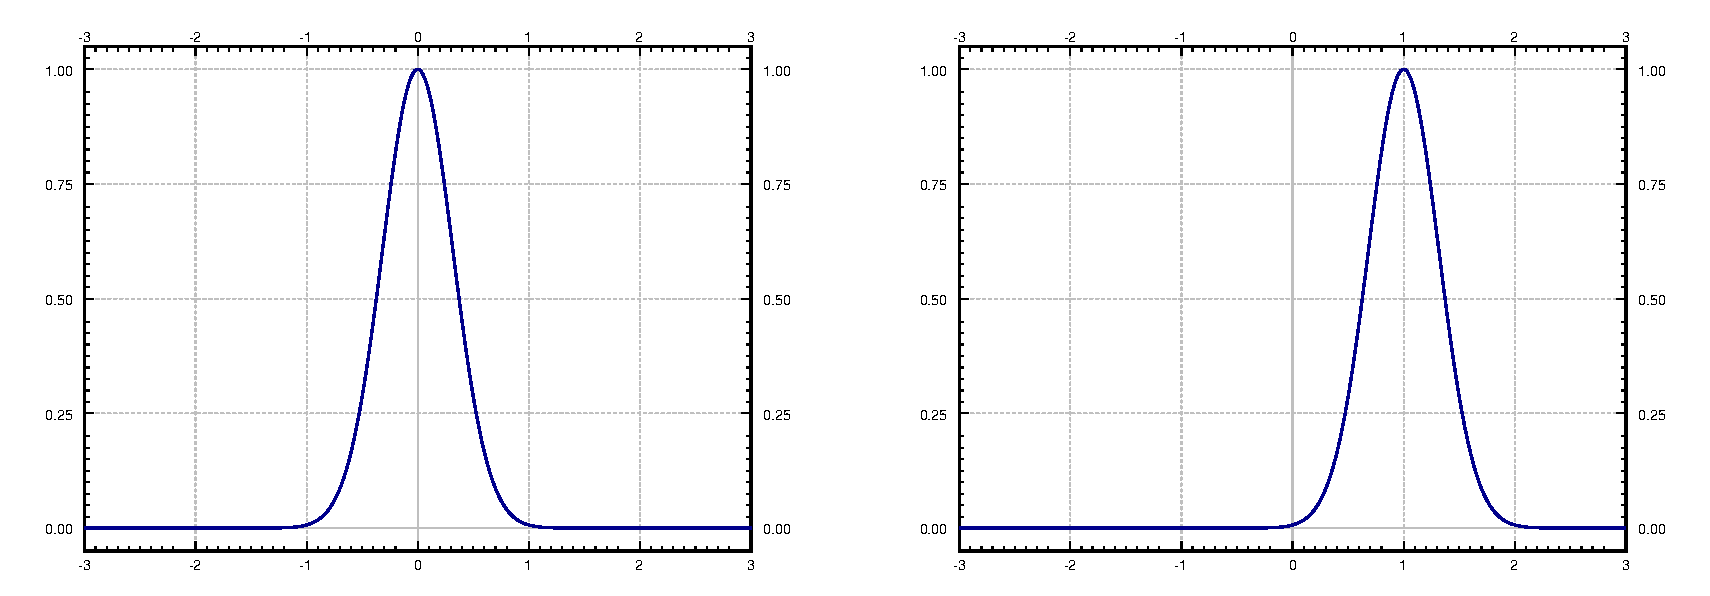
\includegraphics[width=6.24in]{../figures/fopde-transport-1-2}

Example of \myquote{transport}
in $u_t-u_x = 0$ (that is, $\alpha = 1$) where the
initial condition $f(x)$ is a peak at the origin.  On the left is a graph
of the initial condition $u(x,0)$.  On the right is a graph of
the function $u(x,1)$, that is at time $t=1$.  Notice it is the same
graph shifted one unit to
the right.
\end{frame}

\begin{frame}

We use a similar idea in the more general case:
\begin{equation*}
a u_x + b u_t + c u = g, \qquad u(x,0) = f(x)  .
\end{equation*}
We change coordinates to the
characteristic coordinates, which we call $(\xi,s)$.
These are coordinates where $a u_x + b u_t$ becomes differentiation
in the $s$ variable.

Along the characteristic curves (where $\xi$ is constant), we get a
new ODE in the $s$ variable.  In the transport
equation, we got the simple $\frac{du}{ds} = 0$.  In general,
we get the linear equation
\begin{equation}
\frac{du}{ds} + c u = g.
\end{equation}
We think of everything as a function of $\xi$ and $s$,
although
we are thinking of $\xi$ as a parameter rather than an independent variable.
So the equation is an ODE\@.  It is a linear
ODE that we can solve using the integrating factor.

To find the characteristics, think of a curve given parametrically
$\bigl(x(s),t(s)\bigr)$.  We try to have the curve satisfy 
\begin{equation*}
\frac{dx}{ds} = a, \qquad \frac{dt}{ds} = b .
\end{equation*}
Why?
Because when we think of $x$ and $t$ as functions of $s$, we find, using the
chain rule,
\begin{equation*}
\frac{du}{ds} + c u = 
\underbrace{\left( u_x \frac{dx}{ds} + u_t
\frac{dt}{ds}\right)}_{\frac{du}{ds}} + c u =
a u_x + b u_t + c u = g .
\end{equation*}
So we get the ODE {eq:fopde:charode}, which
then describes the value of the solution $u$ of
the PDE along
this characteristic curve.
It is convenient to make sure that $s=0$
corresponds to $t=0$, that is, $t(0) = 0$.  It will also be convenient for
$x(0) = \xi$.
See {fopde:charcurvecurvy}.

\subimport*{../figures/char-curve-curvy.pdf_t}

General characteristic curve.


\begin{example}
Consider
\begin{equation*}
u_x + u_t + u = x, \qquad u(x,0) = e^{-x^2} .
\end{equation*}
We find the characteristics, that is, the curves given by
\begin{equation*}
\frac{dx}{ds} = 1, \qquad \frac{dt}{ds} = 1 .
\end{equation*}
So
\begin{equation*}
x = s + c_1, \qquad t = s+ c_2 ,
\end{equation*}
for some $c_1$ and $c_2$.
At $s=0$, we want $x=\xi$ and $t=0$.  So
we let $c_1 = \xi$ and $c_2 = 0$:
\begin{equation*}
x = s + \xi, \qquad t = s .
\end{equation*}

The ODE is $\frac{du}{ds} + u = x$, and $x = s+\xi$. So, the ODE
to solve along the characteristic is
\begin{equation*}
\frac{du}{ds} + u = s+ \xi .
\end{equation*}
The general solution of this equation, treating $\xi$ as a parameter, is 
$u = C e^{-s}+s+\xi-1$, for some $C$, which can depend on $\xi$.
At $s=0$, our initial condition is that $u$ is
$e^{-\xi^2}$, since at $s=0$, we have $x=\xi$.
Given this initial condition, we find $C=e^{-\xi^2} - \xi +1$.  So,
\begin{equation*}
\begin{split}
u & =
\bigl(e^{-\xi^2} - \xi +1\bigr) e^{-s}+s+\xi-1
\\
& =
e^{-\xi^2-s} + (1 - \xi) e^{-s} +s+\xi-1 .
\end{split}
\end{equation*}
Substitute $\xi = x-t$ and $s=t$ to find $u$ in terms of $x$ and $t$:
\begin{equation*}
\begin{split}
u
& =
e^{-\xi^2-s} + (1 - \xi) e^{-s} +s+\xi-1 
\\
& =
e^{-{(x-t)}^2-t} + (1 - x + t) e^{-t} +x-1 .
\end{split}
\end{equation*}
See {fopde:surfaceplot} for a plot of $u(x,t)$ as a function of
two variables.

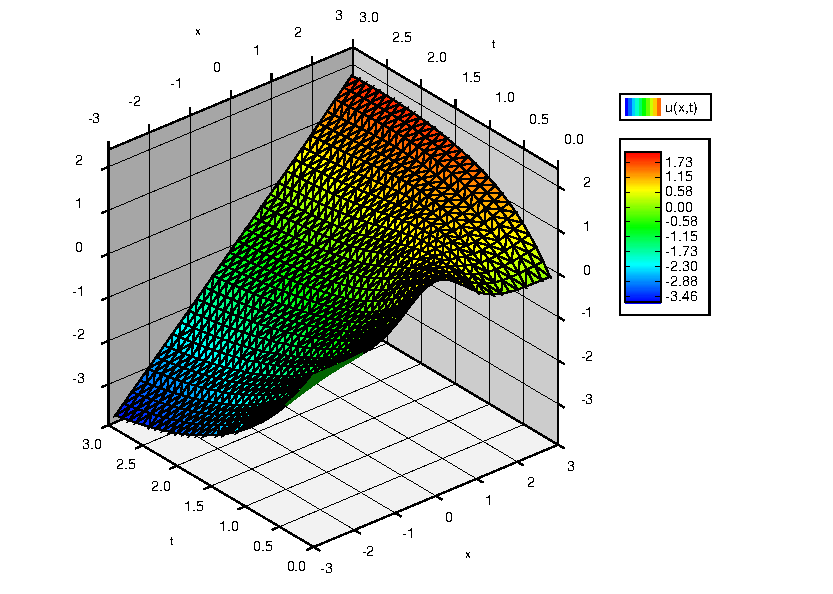
\includegraphics[width=3in]{../figures/sol-to-fo-pde}

Plot of the solution $u(x,t)$ to
$u_x + u_t + u = x$,  $u(x,0) = e^{-x^2}$.
\end{example}

When the coefficients are not constants, the characteristic curves
are not going to be straight lines anymore.

\begin{example}
Consider the following variable coefficient equation:
\begin{equation*}
x u_x + u_t + 2 u = 0, \qquad u(x,0) = \cos(x) . % , \qquad -\infty < x < \infty,
%\quad t > 0 .
\end{equation*}
We find the characteristics, that is, the curves given by
\begin{equation*}
\frac{dx}{ds} = x, \qquad \frac{dt}{ds} = 1 .
\end{equation*}
So
\begin{equation*}
x = c_1 e^{s} , \qquad t = s+ c_2 .
\end{equation*}
At $s=0$, we wish to get $x=\xi$ and $t=0$ as before.  So
\begin{equation*}
x = \xi e^s, \qquad t = s .
\end{equation*}

OK\@, the ODE we need to solve is
\begin{equation*}
\frac{du}{ds} + 2 u = 0 .
\end{equation*}
This is for a fixed $\xi$.  We find $u = C e^{-2s}$.
At $s=0$, we want $u$ to be
$\cos(\xi)$, so that is our initial condition for the ODE.
Moreover, $\xi = xe^{-t}$ and $s=t$.
Consequently,
\begin{equation*}
u = e^{-2s} \cos(\xi)= e^{-2t} \cos(xe^{-t}) .
\end{equation*}
\end{example}


We make a few closing remarks.
One thing to keep in mind is that we would get into trouble if the
coefficient in front of $u_t$, that is the $b$, is ever zero.
Let us consider a quick example of what can go wrong:
\begin{equation*}
u_x + u = 0, \qquad u(x,0) = \sin(x).
\end{equation*}
This problem has no solution.  If we had a solution, it
would imply that $u_x(x,0) = \cos(x)$,
but $u_x(x,0) + u(x,0) = \cos(x) + \sin(x) \not= 0$.
The problem is that the characteristic curve is now the line $t=0$,
and the solution is already provided on that line!

As $b$ ought to then be nonzero,
it is convenient to ensure that $b$ is positive by multiplying
the equation by $-1$
if necessary, so that positive $s$ means positive $t$.

Another remark is that if $a$ or $b$ in the equation are not constants,
the computations can
quickly get out of hand, as the expressions for the characteristic
coordinates become messy and then solving the ODE becomes even messier.
In the examples above, $b$ was always $1$, meaning we got $s=t$ in the 
characteristic coordinates.  If $b$ is not constant, your expression for $s$
will be more complicated.

Finding the characteristic coordinates is really
a system of ODE in general if $a$ depends on $t$ or if $b$ depends on $x$.
In that case, we would need techniques of systems of ODE
to solve, see {sys:chapter} or {nlin:chapter}.  In
general, if $a$ and $b$ are not linear functions or constants, finding closed
form expressions for the characteristic coordinates may be impossible.

Finally, the method of characteristics applies to nonlinear first order PDE
as well.  In the nonlinear case, the characteristics depend not only
on the differential equation, but also on the initial data.  This leads to
not only more difficult computations, but also the formation of
singularities where the solution breaks down at a certain point in time.
An example application where first order nonlinear PDE come
up is traffic flow theory, and you have probably experienced the
formation of singularities: traffic jams.  But we digress.
\end{frame}

\end{document}
